% Description: This file contains the content of the chapter 3 of the dissertation. It is based on an article that me and Grant wrote.

%------------------------------------------------
\chapter{On using Residual H1* for voice quality research} \label{ch:residual_h1}
%------------------------------------------------
%----------------------------------------------------------------------------------------
\section{Introduction} \label{sec:Intro}
%----------------------------------------------------------------------------------------

It is well understood that the term voice quality refers to and describes the manner in which the vocal folds vibrate during speech production. Many languages make use of voice quality to convey paralinguistic information by ``indexing the biological, psychological, and social characteristics of the speaker" \citep{laverVoiceQualityIndexical1968,podesvaStanceWindowLanguageRace2016}. In addition to using voice quality to convey paralinguistic information, many languages use voice quality to convey phonemic distinctions \citep{garellekPhoneticsVoice2019}. 

It has long been established that voice quality contrasts have correlates in the acoustic signal \citep{fischer-jorgensenPhoneticAnalysisBreathy1968,buderAcousticAnalysisVoice1999,kentVoiceQualityMeasurement1999}. For example, \citet{fischer-jorgensenPhoneticAnalysisBreathy1968} found that a strengthened fundamental correlated with breathy voice in Gujarati. In order to normalize the amplitude of the fundamental and counter-act some of the effects of high-pass filtering and differences in sound pressure in the signal, she proposed that you could subtract the amplitude of a higher harmonic, in this case, the second harmonic (H2), from the amplitude of the fundamental (H1). This measure, H1-H2, has since been used in many studies to measure not only breathy voice but other voice quality contrasts as well \citep{garellekPhoneticsVoice2019,chaiH1H2Acoustic2022}.

Despite the large amount of evidence in support of H1-H2, it is not without its problems \citep{chaiH1H2Acoustic2022}. One of the main problems is that using H2 and other normalizations (e.g., H1-A3) are really just attempts at trying to understand the relative strength of the fundamental to higher harmonic energy. Furthermore, \citet{sundbergObjectiveCharacterizationPhonation2022} found that H1 and H2 are affected differently by subglottal pressure, compromising some of the original reasoning behind the use of H1-H2 from \citet{fischer-jorgensenPhoneticAnalysisBreathy1968}. Furthermore, it is not uncommon for researchers to find that H1-H2 is not always the best measure to distinguish voice quality contrasts. For example, \citet{espositoVariationContrastivePhonation2010} found that in Santa Ana del Valle Zapotec H1-H2 was only effective in distinguishing the voice quality contrasts in female speakers of the language and male speakers were better distinguished by H1-A3. Furthermore, \citet{garellekPhoneticsWhiteHmong2021} found that the prominence of the cepstral peak, a type of harmonic measurement of noise, was a better measure to distinguish voice quality contrasts in White Hmong than H1-H2 and other measures of the spectral-slope. 

\citet{chaiH1H2Acoustic2022} found that in addition to the issues mentioned above, errors in measuring H1-H2 is uncomfortably high. This is primarily due to the need to precisely measure two different harmonic amplitudes and when there are errors in calculating H1 this is turn leads to errors in calculating H2 \citep{arrasIntroductionErrorPropagation1998}. An example of this is type of error propagation is that when there are errors in measuring the fundamental frequency, which is especially common with non-modal phonation, errors are introduced into measuring harmonics because they are based on the fundamental. Despite algorithms correcting for vowel height, a common error that occurs with calculating and measuring the fundamental frequency is when a high fundamental frequency co-occurs with a low first formant. This situation causes errors in tracking the fundamental frequency and the first formant. A final issue that can occur with measuring the harmonics is in contexts where the vowel is nasalized. \citet{simpsonFirstSecondHarmonics2012} shows that in these nasalized context, the first nasal pole (P0) can increase the amplitude of H2 and, when the fundamental frequency is  high, H1 is instead increased. 

This collection of errors leads \citet{chaiH1H2Acoustic2022} to propose a new measure, residual H1*. This measure is calculated by first regressing H1 on energy and then subtracting the product of energy and the energy factor from H1. \citeauthor{chaiH1H2Acoustic2022} argue that this measure better reflects the initial purpose of using H1-H2. Furthermore, they find that residual H1*: (i) provides better differentiation between phonation types in !Xóõ; (ii) was more robust for measuring creak in Mandarin with respect to different utterance positions; and (iii) has a stronger relationship to the open quotient than H1*H2*.

For our study, we tested residual H1* with data from Santiago Laxopa Zapotec. This language has a complex interaction between tone and phonation types that has led traditional spectral-tilt measures not adequately to capture the differences in phonation in previous studies. We find that residual H1* can adequately capture differences in voice quality and is a more robust measure of voice quality than H1-H2. Adding credence to the use of this measure in voice quality research. 

The remainder of this paper is organized as follows. Section~\ref{sec:SLZ} provides a brief overview of the Santiago Laxopa Zapotec language. Section~\ref{sec:Methods} describes the methods used in data collection, data processing, and statistical modeling used in this study. Section~\ref{sec:Results} presents the results of the study. Section~\ref{sec:Conclusion} concludes the paper.

%----------------------------------------------------------------------------------------
\section{Santiago Laxopa Zapotec} \label{sec:SLZ}
%----------------------------------------------------------------------------------------
Santiago Laxopa Zapotec is a Northern Zapotec language of the Oto-manguean language family \citep{adlerAcousticsPhonationTypes2016,adlerDerivationVerbInitiality2018,foleyForbiddenCliticClusters2018,foleyExtendingPersonCaseConstraint2020,sichelPronounsAttractionSierra2020, sichelFeaturalLifeNominals2020,brinkerhoffDownstepSantiagoLaxopaMFM,brinkerhoffTonalPatternsTheir2022}. It is spoken by 981 people in the municipality of Santiago Laxopa, Ixtlán, Oaxaca, Mexico \citep{SantiagoLaxopaEconomy} and a small number of other speakers in diaspora throughout Mexico and the United States. Similar to other Oto-manguean languages, Santiago Laxopa Zapotec is laryngeally complex, which refers to how these languages make use of contrastive tone and contrastive voice quality \citep{silvermanLaryngealComplexityOtomanguean1997,silvermanPhasingRecoverability1997,blankenshipTimeCourseBreathiness1997,blankenshipTimingNonmodalPhonation2002}. 

Santiago Laxopa Zapotec exhibits the standard five-vowel inventory, which is further distinguished by the use of a four-way contrast in voice quality. This variety is unique because it is a Northern Core Zapotec that has developed breathy voice in addition to the two types of laryngealization that characterize the rest of the Zapotec languages, namely checked and rearticulated (see \citet{ariza-garciaPhonationTypesTones2018} for a typological study of voice quality distinctions in Zapotec languages).

Santiago Laxopa Zapotec is also tonal with three level tones (H, M, and L) and two contours (MH and HL) appearing in nominals \citep{brinkerhoffTonalPatternsTheir2022}.\footnote{The tonal system of Santiago Laxopa Zapotec for verbs and other lexical categories are still being evaluated.} The language has a complex interaction between tone and phonation types. Every tone can appear with every phonation type, with two exceptions being that breathy voice cannot appear with the high tone and checked voice cannot appear with the rising contour tone.

These interactions between voice quality and tone present a rich environment for testing the reliability of voice quality measures in laryngeally complex languages.

\section{Methods} \label{sec:Methods}
\subsection{Elicitation} \label{sec:Elicitation}

Ten native speakers of SLZ (five female; five male) participated in a wordlist elicitation. Elicitation was performed in the pueblo of Santiago Laxopa, Ixtlán, Oaxaca, Mexico during the summer of 2022 on a Zoom H4n handheld recorder (16-bit, 44.5 kHz). 

The wordlist consisted of 72 items repeated three times each in isolation and the carrier sentence \textit{Shnia' X chonhe lhas} ``I say X three times''. Between these 72 words, there were 11 words with breathy voice, 9 with rearticulated voice, 10 with checked voice, and 42 with modal. Thirteen of the 72 words were disyllabic and contained the same voice quality in each syllable. Of those 13, only five contained mixed voicing.

%----------------------------------------------------------------------------------------
\subsection{Data Processing} \label{sec:DataProcessing}
%----------------------------------------------------------------------------------------

Each vowel of the target words in the carrier sentence condition was labeled following \citet{garellekAcousticDiscriminabilityComplex2020} for where the vowel began and ended. Each vowel in the word list was annotated for speaker, word, vowel, tone, voice quality, and utterance number. This labeling was conducted for each of the vowels located in the target word from the elicitation list of the carrier sentences.

These vowels were then extracted and fed into VoiceSauce for acoustic measuring \citep{shueVoiceSauceProgramVoice2011}. The formants were measured using Snack \citep{sjolanderSnackSoundToolkit2004}, while the fundamental frequency (\textit{f0}) was measured using the STRAIGHT algorithm \citep{kawaharaInstantaneousfrequencybasedPitchExtraction1998}. Spectral slope measures were corrected for formants and bandwidths \citep{hansonGlottalCharacteristicsFemale1997,iseliAgeSexVowel2007}. Each vowel was measured with ten equal time intervals, resulting in 22890 data points in total.

The data was cleaned of outliers following the same steps taken by \citet{chaiH1H2Acoustic2022} in their study. The H1*, H1*–H2*, and \textit{f0} values were z-scored by speaker to reduce the variation between the speakers and provide a way to directly compare the different measures on the same scale. Data points with an absolute z-score value greater than 3 were considered outliers and excluded from the analyzes. Within each vowel category, we calculated the Mahalanobis distance in the F1-F2 panel. Each data point with a Mahalanobis distance greater than 6 was considered an outlier and excluded from the analysis. This is comparable to what was done in \citet{garellekPhoneticsWhiteHmong2021,seyfarthPlosiveVoicingAcoustics2018,chaiCheckedSyllablesChecked2022}. 

Time points whose \textit{f}0, F1, or F2 values were outliers were also excluded from H1* and H1* - H2* analyzes because H1 * and H1 * - H2 * are calculated based on \textit{f}0, F1, and F2. Energy was excluded if it had a value of zero and then log-transformed to normalize its right-skewed distribution. Afterward, the resulted log-transformed data was z-scored and any data point with a z-score larger than 3 was excluded. This outlier removal resulted in 1918 datapoints being removed. 

After the outliers were removed, we calculated residual H1* for the remaining data points following \citet{chaiH1H2Acoustic2022}. First, a linear mixed effects model was generated with the z-scored H1* as the response variable and the z-scored energy as fixed effect. The uncorrelated interaction of the z-scored energy by speaker was treated as random. The energy factor resulting from this linear mixed-effects model was extracted. Finally, the z-scored H1* had the product of the z-scored energy and the energy factor subtracted from it, giving us the residual H1* measure.

The measures were then assigned according to their position in the vowel (first, middle, and third) for statistical modeling.  

%----------------------------------------------------------------------------------------
\subsection{Statistical modeling} \label{sec:StatisticalModeling}
%----------------------------------------------------------------------------------------

Three linear mixed-effects regression models were fitted, one each for the z-scored H1*-H2* and residual H1*. Each model had tone and interaction between voice quality and position in the vowel as fixed effects, and vowel and interaction between speaker, word, and repetition as random intercepts.

\begin{equation}
  Measure \sim  Phonation*Position + Tone + (1|Speaker:Word:Repetition) + (1|Vowel) 
\end{equation}

The tone and the interaction between voice quality and position in the vowel were selected as fixed effects for several reasons. The first is that five unique tones appeared in the data and it is well established that tone interacts with voice quality in different ways (see \cite{espositoCrossLinguisticPatterns2020,garellekPhoneticsVoice2019} for discussion). By treating tone as a fixed effect in our model, we can account for these interactions. The interaction between voice quality and position in the vowel as a fixed effect was included to account for the temporal differences that between the two different laryngealizations; checked and rearticulated vowels. Checked vowels in Zapotec languages have a glottal occlusion or a short period of creaky voice located at the right edge of the vowel. This is in contrast to rearticulated vowels, where there is a glottal occlusion or creaky voice in the middle of the vowel. Because this difference between checked and rearticulated vowels is temporal in nature, we can account for this difference through the interaction of voice quality and position in the vowel.\footnote{Tone and voice quality are closely linked . By including only the positional interaction with voice quality we can avoid collinear interactions that appear when we try to include tone in the interaction.}

The interaction between speaker, word, and repetition was treated as a random intercept because this allows us to take into account that each speaker said each word on the elicitation list three times. This intercept accounts for not only the intra-speaker variability, but also the inter-speaker variability during each time the word was uttered. Treating a vowel as a random intercept allows us to capture the fact that each voice quality occurred with different vowels during elicitation.

%----------------------------------------------------------------------------------------
\section{Results} \label{sec:Results}
%----------------------------------------------------------------------------------------
%----------------------------------------------------------------------------------------
\subsection{H1*-H2*} \label{sec:H1H2}
%----------------------------------------------------------------------------------------

Figure~\ref{fig:FIG1} shows the mean H1*-H2* values for each voice quality at each of the ten vowel intervals. We see that the breathy, checked, and rearticulated all have values lower than the modal at each of the first nine intervals. In the final interval, breathy and rearticulated are essentially equal to the modal value. In contrast, checked's value remains lower than the modal's value throughout the entire vowel.

\begin{figure}[htbp]
  \centering
  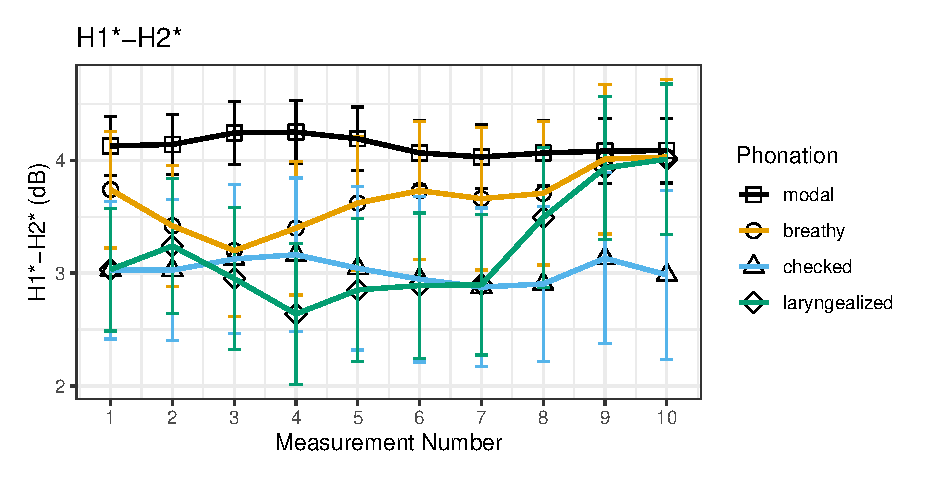
\includegraphics[width = 0.75\textwidth]{images/Figure1.eps}
  \caption{\label{fig:FIG1}{H1*-H2* across the duration of the vowel. Points represent the mean of each measure across the ten intervals. The error bars around each point represent ±1.96 Std. Error. A line was plotted over each to show how the acoustic measure functions across the ten intervals.}}
\end{figure}

% \begin{table}[!h]
%   \centering
%   \caption{Results of the linear mixed-effects model for z-scored H1*-H2*.}
%   \label{tab:H1H2Results}
%   \begin{ruledtabular}
%   \begin{tabular}{lrrrrrl}
%       & Estimate & Std. Error & df & t-value & p-value & \\ \hline
%     \textit{(Intercept)} & 0.02876 & 0.09336 & 6.17877 & 0.30809 & 0.76814 & \\
%     Breathy & -0.03569 & 0.04210 & 9749.84999 & -0.84781 & 0.39656 & \\
%     Checked & -0.14120 & 0.04050 & 14402.97700 & -3.48623 & \textless 0.001 & ***\\
%     Rearticulated & -0.13719 & 0.04964 & 5353.41205 & -2.76340 & 0.00574 & **\\
%     Position 2 & 0.00475 & 0.01339 & 19027.80227 & 0.35456 & 0.72293 & \\
%     Position 3 & -0.01795 & 0.01259 & 19039.57085 & -1.42613 & 0.15385 & \\
%     Tone H & 0.01597 & 0.04454 & 4340.72994 & 0.35855 & 0.71995 & \\
%     Tone L & -0.07794 & 0.03218 & 8176.59285 & -2.42248 & 0.01544 & *\\
%     Tone M & -0.10568 & 0.04397 & 7428.42296 & -2.40365 & 0.01626 & *\\
%     Tone R & 0.28710 & 0.06918 & 10218.05414 & 4.15025 & \textless 0.001 & ***\\
%     Breathy:Position 2 & 0.02104 & 0.03069 & 19046.99970 & 0.68566 & 0.49294 & \\
%     Checked:Position 2 & -0.00034 & 0.03597 & 19063.65965 & -0.00949 & 0.99242 & \\
%     Rearticulated:Position 2 & -0.06258 & 0.03226 & 19036.21224 & -1.94021 & 0.05237 & .\\
%     Breathy:Position 3 & 0.16346 & 0.02900 & 19087.82852 & 5.63588 & \textless 0.001 & ***\\
%     Checked:Position 3 & 0.04822 & 0.03400 & 19096.31688 & 1.41845 & 0.15608 & \\
%     Rearticulated:Position 3 & 0.14092 & 0.03025 & 19072.44284 & 4.65848 & \textless 0.001  & ***\\
%   \end{tabular}
%   \end{ruledtabular}
% \end{table}

%----------------------------------------------------------------------------------------
\subsection{Residual H1*} \label{sec:ResidH1}
%----------------------------------------------------------------------------------------

Figure~\ref{fig:FIG2} shows the mean residual H1* values for each voice quality at each of the ten vowel intervals. In contrast to Figure~\ref{fig:FIG1}, we see that breathy has a higher residual H1* measure than modal throughout the duration of the vowel, which is consistent with other observations for breathy voice \citep{fischer-jorgensenPhoneticAnalysisBreathy1968}. Checked and rearticulated both have lower values than the modal at each of the 10 intervals. In addition, it shows that the checked voice has a lower residual H1 * value than the rearticulated voice at intervals 8 through 10. The rearticulated voice has a lower residual H1 * value than the checked voice at intervals 1 through 7, showing the temporal distinction between these two voice qualities. 

\begin{figure}[htbp]
  \centering
  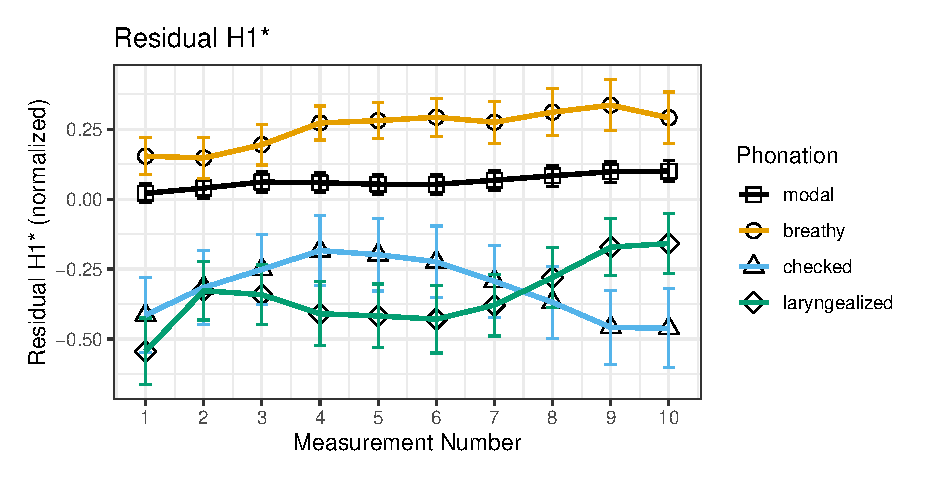
\includegraphics[width = 0.75\textwidth]{images/Figure2.eps}
  \caption{\label{fig:FIG2}{Residual H1* across the duration of the vowel. Points represent the mean of each measure across the ten intervals. The error bars around each point represent ±1.96 Std. Error. A line was plotted over each to show how the acoustic measure functions across the ten intervals.}}
\end{figure}

% \begin{table}[!h]
%   \centering
%   \caption{Results of the linear mixed-effects model for Residual H1*.}
%   \label{tab:ResH1Results}
%   \begin{ruledtabular}
%   \begin{tabular}{lrrrrrl}
%     & Estimate & Std. Error & df & t-value & p-value & \\ \hline 
%     \textit{(Intercept)} & -0.10483 & 0.04015 & 10.71725 & -2.61084 & 0.02469 & *\\
%     Breathy & 0.14997 & 0.03175 & 5393.82513 & 4.72315 & \textless 0.001 & ***\\
%     Checked & -0.38554 & 0.03061 & 5905.98167 & -12.59335 & \textless 0.001 & ***\\
%     Rearticulated & -0.48437 & 0.03740 & 4633.21778 & -12.95239 & \textless 0.001 & ***\\
%     Position 2 & 0.01369 & 0.01027 & 19029.30204 & 1.33294 & 0.18257 & \\
%     Position 3 & 0.04386 & 0.00966 & 19041.55355 & 4.54158 & \textless 0.001 & ***\\
%     Tone H & 0.09272 & 0.03335 & 2975.18807 & 2.78046 & 0.00546 & **\\
%     Tone L & 0.18568 & 0.02439 & 7860.40311 & 7.61295 & \textless 0.001 & ***\\
%     Tone M & 0.05475 & 0.03328 & 7005.78449 & 1.64525 & 0.09996 & .\\
%     Tone R & 0.33507 & 0.05257 & 9813.69066 & 6.37372 & \textless 0.001 & ***\\
%     Breathy:Position 2 & 0.11599 & 0.02354 & 19049.14884 & 4.92755 & \textless 0.001 & ***\\
%     Checked:Position 2 & 0.10060 & 0.02759 & 19066.47122 & 3.64602 & \textless 0.001 & ***\\
%     Rearticulated:Position 2 & -0.02675 & 0.02474 & 19038.08812 & -1.08092 & 0.27975 & \\
%     Breathy:Position 3 & 0.11491 & 0.02225 & 19091.32792 & 5.16510 & \textless 0.001 & ***\\
%     Checked:Position 3 & -0.10327 & 0.02608 & 19100.43388 & -3.96047 & \textless 0.001 & ***\\
%     Rearticulated:Position 3 & 0.12029 & 0.02320 & 19075.58487 & 5.18437 & \textless 0.001 & ***\\
%   \end{tabular}
%   \end{ruledtabular}
% \end{table}

%----------------------------------------------------------------------------------------
\subsection{Model Comparison} \label{sec:Comparison}
%----------------------------------------------------------------------------------------

In order to asses the robustness of the models we compared the residual H1* linear mixed-effects model to the H1*-H2* linear mixed-effects model. This was carried out using two methods: direct comparison of the outputs of the two models in the same way as \citet{chaiH1H2Acoustic2022} and the Akaike Information Criterion (AIC). 

Table~\ref{tab:CGComparison} shows the results of the comparison of the linear mixed-effects models for H1*-H2* and residual H1 *. In comparing these models, we find that the residual H1* model performed better than the H1*-H2* model in distinguishing voice quality contrasts in Santiago Laxopa Zapotec. This is supported by the larger absolute value of the coefficient estimate, the lower standard error and the higher t-value of the residual H1* to distinguish breathy, checked and rearticulated vowels from modal vowels.

\begin{table}[!h]
  \centering
  \caption{Model comparison between H1*–H2* and Residual H1* in distinguishing Santiago Laxopa Zapotec voice quality.}
  \label{tab:CGComparison}
%   \begin{ruledtabular}
    \begin{tabular}{lllllll}
    Voice Quality Contrast & Model & \textit{$\beta$ } & Std. Error & \textit{t}-value & \textit{p}-value  &     \\
    \hline
      Breathy vs Modal &  H1*-H2* & -0.03569    & 0.04210         & -0.84781  & 0.39656 & \\
      & Res. H1* & 0.14997  & 0.03175 & 4.72315   & \textless 0.001   & *** \\
      Checked vs Modal & H1*-H2* & -0.14120    & 0.04050         & -3.48623  & \textless 0.001 & *** \\
      & Res. H1* & -0.38554 & 0.03061 & -12.59335 & \textless 0.001 & *** \\
      Rearticulated vs Modal & H1*-H2 & -0.13719   & 0.04964         & -2.76340 & 0.00574           & **  \\
     & Res. H1* & -0.48437 & 0.03740 & -12.95239 & \textless 0.001 & *** \\
    \end{tabular}
%   \end{ruledtabular}
\end{table}

Table~\ref{tab:Comparison} shows the results of the AIC comparison between the H1*-H2* and residual H1* models. The residual H1* model had a lower AIC than the H1 * -H2 * model, indicating that the residual H1* model is a better fit for the data than the H1*-H2* model. Even though AIC comparison is usually conducted on nested models, it is still a useful tool for comparing non-nested models \citep{burnhamMultimodelInferenceUnderstanding2004,burnhamAICModelSelection2011,burnhamModelSelectionMultimodel2004}.

\begin{table}[!h]
  \centering
  \caption{AIC for the H1*-H2* and residual H1* models.}
  \label{tab:Comparison}
%   \begin{ruledtabular}
  \begin{tabular}{lll}
    Model  & AIC & $\Delta$ AIC\\
    \hline
    H1*-H2* model & 43386.99 & 11214.54 \\
    Residual H1* model & 32172.45 & 0 \\
  \end{tabular}
%   \end{ruledtabular}
\end{table}
%% Before bibliography:

\section{Conclusion} \label{sec:Conclusion}

In conclusion, we find that residual H1* is a more robust measure of voice quality than H1-H2 in Santiago Laxopa Zapotec. This is supported by the results of the linear mixed-effects models, which show that residual H1* is better at distinguishing breathy, checked, and rearticulated vowels from modal vowels. This is further supported by the AIC comparison, which shows that the residual H1* model is a better fit for the data than the H1*-H2* model. These results lend credence to the claims of \citet{chaiH1H2Acoustic2022} and support the use of residual H1* in voice quality research, especially in laryngeally complex languages.